\chapter{Über diese \LaTeX{}-Vorlage}
Diese Vorlage ersetzt eine ältere Vorlage, die ich auf Basis von Professor Klaus Dohmens Vorlage erstellt hatte. Nachfolgend finden Sie einige wichtige Informationen zu dieser aktuellen Vorlage vom Mai 2025. Eine gute und umfassende Einführung in \LaTeX{} finden sie im \href{https://de.wikibooks.org/wiki/LaTeX-Kompendium}{LaTeX-Kompendium}. Eine superkurze Einführung ist auch in meinem Buch \textit{Angewandte Bioinformatik} ( \cref{fig:latex}) enthalten \citep{Wuenschiers2016kap12}.

\begin{figure}[h]
    \centering
    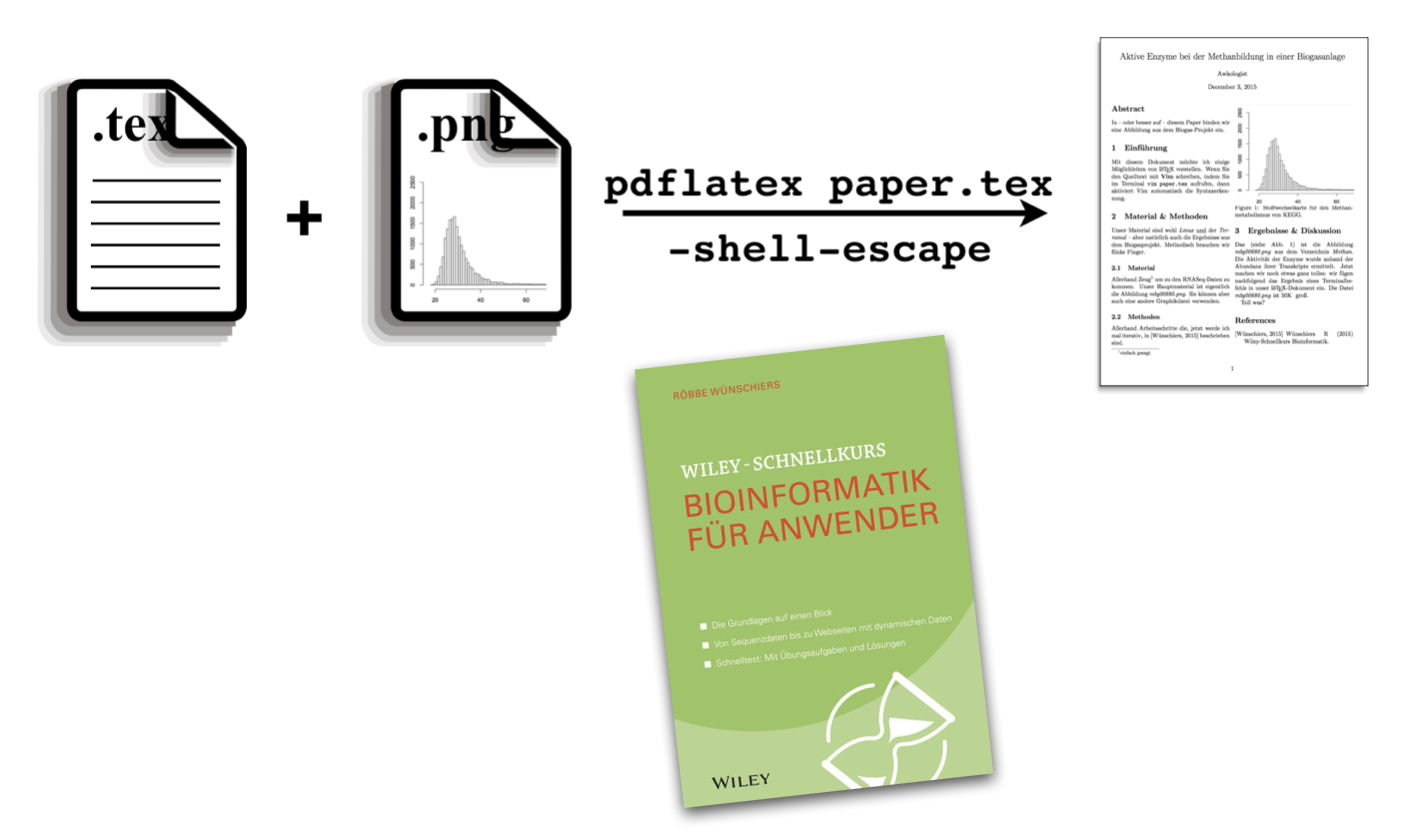
\includegraphics[width=.7\columnwidth]{fig-latex.png}
    \caption{Von \LaTeX{} zum PDF. Aus \citep{Wuenschiers2016}}.
    \label{fig:latex}
\end{figure}

Scheuen Sie sich nicht, mich auf Fehler hinzuweisen und Verbesserungsvorschläge einzubringen: \href{mailto:rw@biowasserstoff.de?subject=HSMW LaTeX-Vorlage}{Email}.

\alertinfo{Diese Beschreibung ist noch in Arbeit. Aktueller Stand: \today}

\section{Notwendige Software}
Wenn Sie es sehr komfortabel haben möchten, dann arbeiten Sie in \href{https://www.overleaf.com}{Overleaf}. Um diese Vorlage zu verwenden, reicht die kostenlose Version aber nicht aus und Sie müssen als Student:in derzeit 8€ zahlen.

Wenn Sie Overleaf verwenden, müssen Sie zum kompilieren (PDF-Erstellung) LuaLaTeX einstellen (\cref{fig:overleaf}).

\begin{figure}[h]
\centering
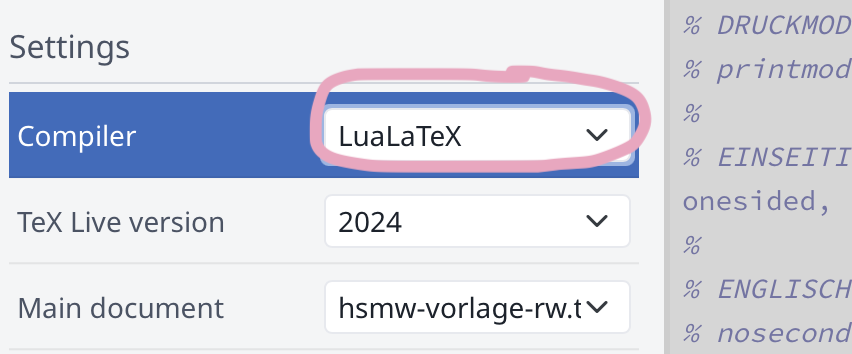
\includegraphics[width=.5\columnwidth]{overleaf.png}
\caption{Einstellung von LuaLaTeX als Compiler im Menu von Overleaf.}.
\label{fig:overleaf}
\end{figure}

Alternativ können Sie bspw. \href{https://www.xm1math.net/texmaker/}{TexMaker} lokal auf ihrem Computer installieren. Texmaker ist aber nur ein Editor. Um mit LaTeX zu arbeiten, benötigen Sie neben dem Editor eine LaTeX-Distribution (texlive oder miktex auf Windows, texlive auf Linux, mactex auf Mac). Die Installation von TexMaker mit Miktex ist \href{https://youtu.be/uKetjJTDSqk}{hier} erklärt.

In \cref{fig:texmaker} ist eine wichtige Einstellung gezeigt: Anstelle des veralteten \texttt{pdflatex} (hat u.a. Probleme mit Unicode), verwenden wir das moderne \texttt{lualatex}. Das Programm \texttt{biber} kümmert sich um die Literatur. Die Befehlsoption \texttt{-synctex=1} bewirkt, dass das PDF- und Tex-Dokument synchronisiert werden. Ein Rechtsklick mit der Maus im jeweiligen Fenster erlaubt den Sprung an die entsprechende Stelle. Nice.

\begin{figure}[h]
\centering
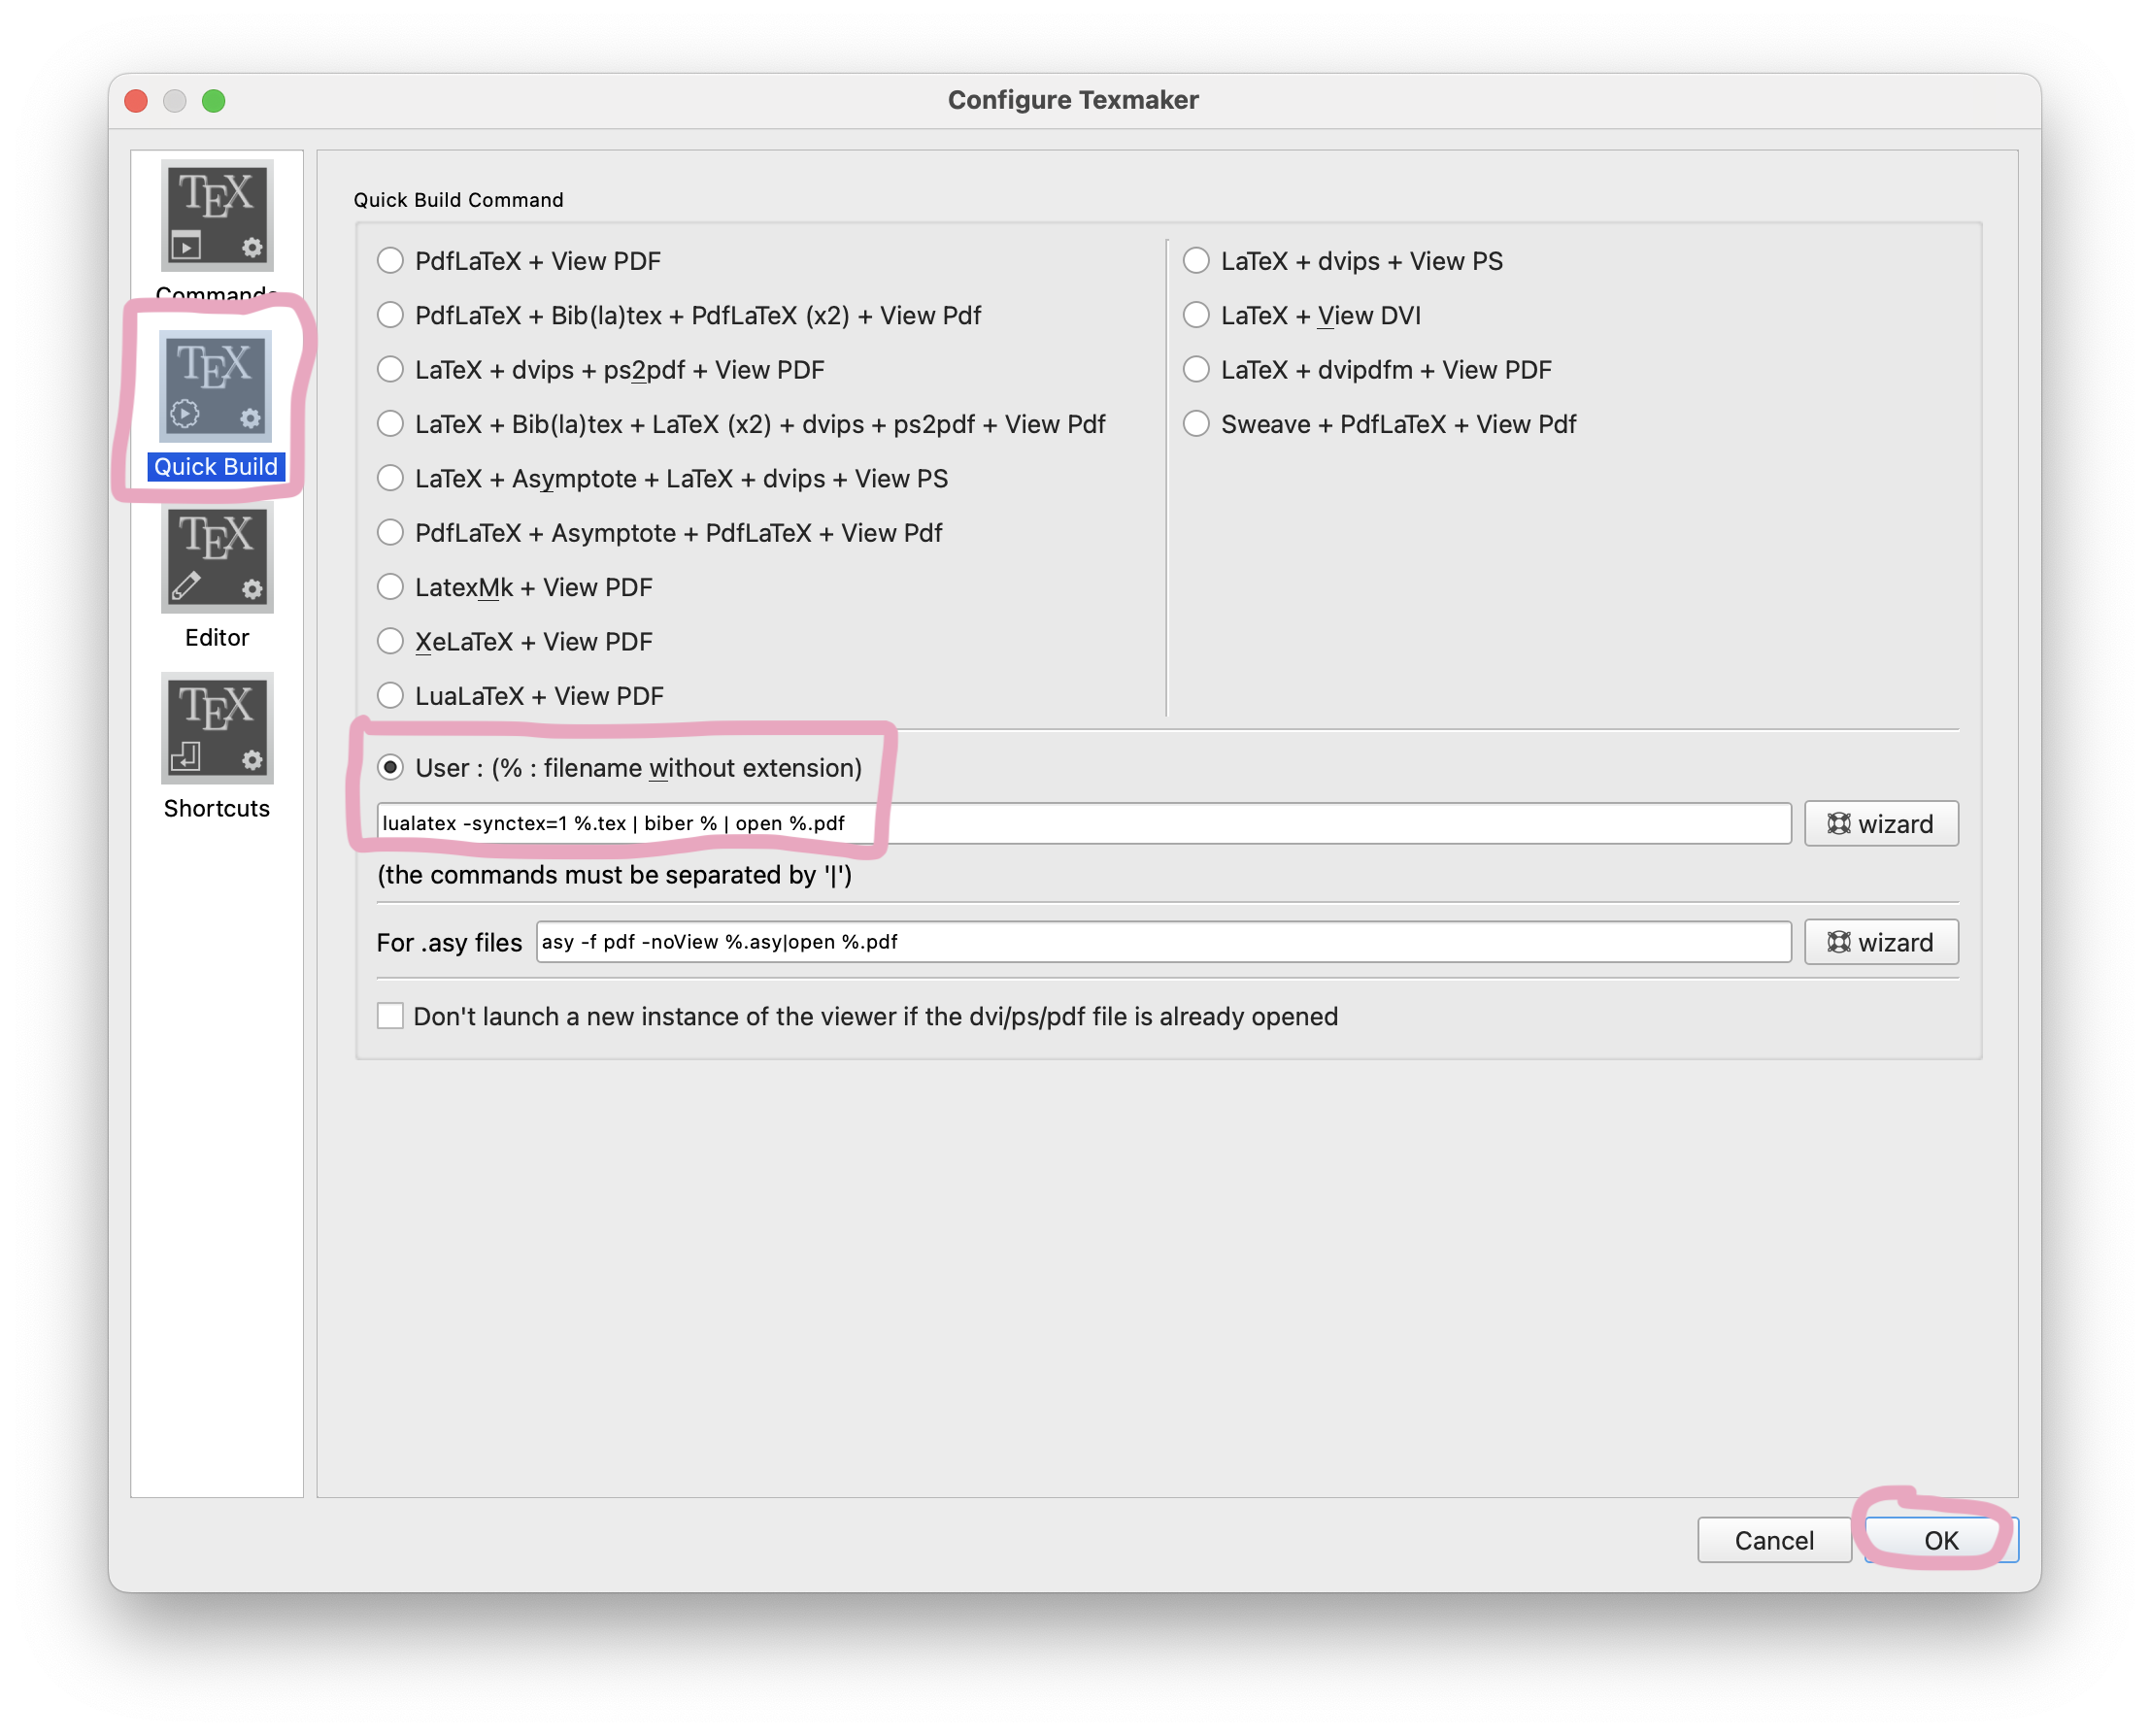
\includegraphics[width=.7\columnwidth]{texmaker.png}
\caption{Der Befehl \texttt{lualatex -synctex=1 \%.tex | open \%.pdf} sollte für die Erstellung des PDFs verwendet werden. Dies legen Sie in den Einstellungen fest.}.
\label{fig:texmaker}
\end{figure}

\section{Notwendige Dateien}
Diese Vorlage besteht aus mehreren Dateien, die alle im selben Verzeichnis liegen müssen. Sie können diese von meinem \href{https://github.com/awkologist/HSMW-Template-BioChem-Group}{GitHub-Repository} nach Klick auf den Button \verb+<>Code+ und \textit{Download ZIP} als Dateiarchiv herunterladen und dann entweder in

\begin{itemize}
 \item \href{https://www.overleaf.com}{Overleaf} unter \textit{New Project} $\rightarrow$ \textit{Upload Project} oder
 \item TexMaker
\end{itemize}  
 
importieren. Die Dateien sind ...

\begin{tabular}{lp{.6\textwidth}}
\textit{hsmw-vorlage-rw.tex} & Die Hauptdatei, die die Formatierung bestimmt und Grunddaten enthält \\
\textit{mein-text.tex} & Datei, die ihren Haupttext enthält \\
\textit{fig-latex.png} & Eine Abbildung als Beispiel\\
\textit{magic-juggler.png} & Ein Logo als Beispiel\\
\textit{unterschrift.jpg} & Eine Unterschrift für die Selbstständigkeitserklärung als Beispiel\\
\textit{meine-abk.tex} & Datei mit den Begriffen und Definitionen für das Abkürzungsverzeichnis\\
\textit{meine-literatur.txt} & Datei mit ihrer Literatur im Bibtex-Format\\
\textit{hsmw-vorlage-rw.cls} & Die Style-Datei, welche die Formatierung bestimmt $\rightarrow$ \textbf{nicht editieren}\\
\textit{hsmw-biblatex.cfg} & Konfiguration für Literaturverzeichnis  $\rightarrow$ \textbf{nicht editieren}\\
\end{tabular}

\section{Wie passe ich die Dateien an?}
Als ersten bearbeiten Sie die Datei \textit{hsmw-vorlage-rw.tex}. In der ersten Zeile wird die Dokumentenklasse \textit{hsmw-vorlage-rw} mit 

\verb+\documentclass[OPTIONEN]{hsmw-vorlage-rw}+ 

aufgerufen. Dabei stehen Ihnen zahlreichen OPTIONEN (Klassenoptionen) zur Verfügung, die in der Datei \textit{hsmw-vorlage-rw.tex} aber auch im nachfolgenden Kapitel beschrieben sind.

\alertinfo{Achten Sie auf die besondere Funktion des Prozentzeichens (\%). Es initiiert einen Kommentar, d.h. nachfolgender Text wird nicht als LaTeX interpretiert. }


\chapter{Verfügbare Optionen und Befehle}
\label{cha:optionsAndCommands}
	
Im Folgenden finden Sie eine Auflistung verfügbarer Klassenoptionen und Befehle, die direkte Auswirkungen auf die Dokumentenvorlage haben.

Die wichtigste Entscheidung zu Beginn ist, ob Sie das Format für ein Protokoll, einen Beleg oder eine Abschlussarbeit verwenden wollen. 
In der Datei \textit{hsmw-vorlage-rw.tex} legen Sie fest, um welchen Dokumententyp es sich handelt.
	
\section{Klassenoptionen}
\label{sec:klassenoption}
	
Die Klassenoptionen dienen der initialen Konfiguration der Vorlage und sollten entsprechend zu Beginn des Dokuments gewählt werden, wenn eine Abweichung vom vordefinierten Standardverhalten gewünscht ist.

% Einige der Optionen sind voneinander abhängig oder beeinflussen sich gegenseitig, weswegen deren vorgeschlagene Reihenfolge nicht verändert werden sollte, um Fehler zu vermeiden.

Einige Optionen nehmen Werte entgegen, andere dienen nur als Schalter (on/off) und besitzen keine zusätzlichen Parameter. Letztere sind also entweder vorhanden oder auskommentiert.

Nachfolgende Liste enthält nur die wichtigsten Optionen.

\begin{tabular}{lp{.6\textwidth}}
\textbf{\texttt{language}} & \textit{english}, \textit{german} $\rightarrow$ Lädt die Standardsprache für das Dokument \\

\textbf{\texttt{thesis}} & \textit{protokoll}, \textit{beleg}, \textit{bachelor}, \textit{master}, \textit{paper}, \textit{shortpaper}, \textit{diploma} $\rightarrow$ Schaltet die Art der Vorlage um (Beleg oder Abschlussarbeit) und setzt Standardbezeichnungen und Layouteinstellungen\\

\textbf{\texttt{printmode}} & \textit{on/off} $\rightarrow$ Verbirgt farbige Hyperlinks im Dokument und ändert die Farbdefinitionen zur Druckoptimierung ins CMYK-Farbmodell \\

\textbf{\texttt{onesided}} & \textit{on/off} $\rightarrow$ Wechselt zum einseitigen Dokumentenformat; bspw. sind alle Seitenzahlen rechtsbündig. \\

\textbf{\texttt{nosecondtitle}} & \textit{on/off} $\rightarrow$ Verbirgt die zweite englischsprachige Titelseite bei Abschlussarbeiten \\

\textbf{\texttt{compactlistof}} & \textit{on/off} $\rightarrow$ Abbildungs-, Tabellen- und Abkürzungsverzeichnis beginnen nicht auf separaten Seiten \\

\textbf{\texttt{noauthorship}} & \textit{on/off} $\rightarrow$ Verbirgt die Selbstständigkeitserklärung bzw. Eidesstattliche Erklärung \\

\textbf{\texttt{lotbeforelof}} & \textit{on/off} $\rightarrow$ Tauscht die Reihenfolge des Abbildungs- und Tabellenverzeichnisses \\

\textbf{\texttt{graduatedtoc}} & \textit{on/off} $\rightarrow$ Erstellt ein eingerücktes Inhaltsverzeichnis \\

\textbf{\texttt{colorlinks}} & \textit{on/off} $\rightarrow$ Verwendet farbige Hyperlinks im Dokument \\

\textbf{\texttt{acronymhref}} & \textit{on/off} $\rightarrow$ Schaltet Hyperlinks zum Abkürzungsverzeichnis an oder aus \\

\textbf{\texttt{acronymdots}} & \textit{on/off} $\rightarrow$ Schaltet die Punktlinie im Abkürzungsverzeichnis an oder aus \\

\textbf{\texttt{fancy}} & \textit{on/off} $\rightarrow$ ] Ändert mehrere Stiloptionen in Annäherung an das Corporate Design der Hochschule \\

\textbf{\texttt{faculty}} & \textit{inw}, \textit{cb}, \textit{wi}, \textit{sw}, \textit{me} $\rightarrow$  Lädt einen vordefinierten Fakultätsnamen \\

\end{tabular}

\alertinfo{Im \textbf{zweiseitigen Layout} versucht LaTeX einen einheitlichen Abschluss für die Ober- und Unterkante des Texts zu setzen, damit die Seiten im gedruckten Zustand gut zum Seitenrand hin abschließen. Dies funktioniert gut für Dokumente mit viel Text, kann allerdings in Kombination mit Abbildungen, Tabellen oder vielen kurzen Kapiteln / Abschnitten zu einem lückenhaften Layout führen. Um dieses zu vermeiden kann der Schalter \enquote{\textit{\string\raggedbottom}} in der Präambel gesetzt werden (Standardverhalten für zweiseitiges Layout: \textit{\string\flushbottom})}

	
\section{Individuelle Daten eintragen}
\label{sec:macros}
In \cref{tab:macros} ist eine Übersicht vordefinierter Befehle für die individuelle Konfiguration der Vorlage gegeben.
Je nach gewähltem Dokumententyp (Protokoll, Beleg, Abschlussarbeit, etc.) und gewünschtem Dokumentenaufbau ist nur eine Auswahl davon nötig.

\alertinfo{Sollten einzelne Angaben fehlen, werden diese im generierten PDF rot hervorgehoben.}

Einige der Befehle haben einen oder mehrere optionale Parameter, die im Folgenden kurz erläutert werden. Konkrete Anwendungsbeispiele entnehmen Sie bitte der Datei \textit{hsmw-vorlage-rw.tex}.
	
	\begin{table}[!htb]
		\def\yes{notwendig}
		\def\no{-}
		\def\maybe{optional}
		
		\centering
		\caption{Verfügbare Befehle und deren Anwendungszwecke nach Dokumententyp.}
		\label{tab:macros}
		\begin{tabular}{llll}
			\toprule
			\textbf{Beschreibung} & \textbf{Beleg} & \textbf{Abschlussarbeit} & \textbf{Befehl(e)} \\
			\midrule
\hyperref[cmd:type]{Art des Dokuments} & \yes & \yes & \texttt{type} \\
			\hyperref[cmd:author]{Autor(en)} & \yes & \yes & \texttt{author}, \texttt{addauthor} \\
			\hyperref[cmd:title]{Titel} & \yes & \yes & \texttt{title} \\
			\hyperref[cmd:subtitle]{Untertitel} & \maybe & \maybe & \texttt{subtitle} \\
			\hyperref[cmd:submissiondate]{Abgabedatum} & \yes & \yes & \texttt{submissiondate} \\
			\hyperref[cmd:defensedate]{Verteidigungsdatum} & \no & \yes & \texttt{defensedate} \\
			\hyperref[cmd:location]{Ort der Unterschrift} & \maybe & \maybe & \texttt{location} \\
			\hyperref[cmd:date]{Datum der Unterschrift} & \maybe & \maybe & \texttt{date} \\
			\hyperref[cmd:faculty]{Fakultät} & \maybe & \yes & \texttt{faculty} \\
			\hyperref[cmd:courseofstudy]{Studiengang} & \maybe & \yes & \texttt{courseofstudy} \\
			\hyperref[cmd:module]{Modul} & \maybe & \no & \texttt{module} \\
			\hyperref[cmd:seminargroup]{Seminargruppe} & \maybe & \yes & \texttt{seminargroup} \\
			\hyperref[cmd:email]{E-Mail} & \maybe & \no & \texttt{email} \\
\hyperref[cmd:examiner]{Prüfer} & \maybe & \yes & \texttt{examiner}, \texttt{addexaminer} \\
\hyperref[cmd:betreuer]{Betreuer} & \maybe & \maybe & \texttt{betreuer} \\
			\hyperref[cmd:abstract]{Referat} & \no & \yes & \texttt{abstract} \\
			\hyperref[cmd:preface]{Vorwort} & \no & \maybe & \texttt{preface} \\
			\hyperref[cmd:dedication]{Danksagung} & \no & \maybe & \texttt{dedication} \\
			\hyperref[cmd:nda]{Sperrvermerk} & \no & \maybe & \texttt{nda} \\
			\hyperref[cmd:frontispiece]{Frontispiz} & \no & \maybe & \texttt{frontispiece} \\
			\hyperref[cmd:partnerlogo]{Partnerlogo} & \maybe & \maybe & \texttt{partnerlogo} \\
			\bottomrule
		\end{tabular}
	\end{table}
	
\textbf{Art des Dokuments:}\phantomsection\label{cmd:type}
Schreibt den Dokumententyp auf den Titelseiten und in den bibliografischen Angaben. Er wird eigentlich durch die Klassenoption (siehe \cref{sec:klassenoption}) festgelegt, kann aber mit diesem Befehl (\texttt{type}) überschrieben werden.

\textbf{Autor:}\phantomsection\label{cmd:author}
Setzt den Autor auf den Titelseiten, den bibliografischen Angaben und der Selbstständigkeitserklärung. Für den ersten Autor nutzen Sie bitte \verb|\author| und für zusätzliche Autoren \verb|\addauthor|. Die vollständige Befehlssyntax beider Befehle ist:


{\small\verb|\author*(Anrede)[Titel]{Vorname}{Nachname}[Akad. Grad]<Unterschrift><Shift>|}
	\begin{itemize}
		\item Optional: *Sternversion schaltet zwischen der weiblichen und männlichen Anrede (Herr oder Frau) und passenden Labels (Autor wird zu Autorin) um
		\item Optional: (Anrede) überschreibt die vordefinierte Standardanrede (Herr bzw. Frau)
		\item Optional: [Titel] vor dem Vornamen (z.\,B. Dr. oder Prof. Dr. rer. nat.)
		\item Vorname
		\item Nachname
		\item Optional: [Akad. Grad] hinter dem Nachnamen (z.\,B. M.A. oder B.Sc.)
		\item Optional: <Unterschrift> gibt den Pfad zu einer Unterschriften-Datei an\footnote{Sollten Ihnen die Unterschriften in der Selbstständigkeitserklärung zu klein wirken, können Sie diese mit dem Befehl \texttt{\textbackslash{}setlength\{\textbackslash{}signatureHeight\}\{3\textbackslash{}baselineskip\}} in der Präambel vergrößern.}
		\item Optional: <Shift> schiebt die Unterschrift nach unten (z.\,B. \textit{0.5cm})
	\end{itemize}\vspace*{-\baselineskip}
	Beispiele für Autorenangaben:
	\begin{itemize}
		\item Ohne Titel und akademische Grade
		\begin{itemize}
			\item Männlicher Autor: \verb|\author{Holger Amadeus}{Herzog}|
			\item Weibliche Autorin: \verb|\author*{Frieda}{Fröhlich}|
			\item Mit Unterschrift: \verb|\author*{Frieda}{Fröhlich}<signatur-frieda.pdf>|
		\end{itemize}
		\item Mit Titel oder akademischen Grad
		\begin{itemize}
			\item Professor: \verb|\author[Prof.]{Egon}{Engelsbach}|
			\item Doktorin: \verb|\author*[Dr. rer. nat.]{Lucy}{Landgraf}<lucy.pdf>|
			\item Bachelorabschluss: \verb|\author{Sven}{Svenson}[B.Sc.]|
		\end{itemize}
		\item Mehrere Autoren:
		\begin{itemize}
			\item \verb|\author{Holger Amadeus}{Herzog}|
			\item \verb|\addauthor*{Frieda}{Fröhlich}<signatur-von-frieda.pdf>|
			\item \verb|\addauthor{Sven}{Svenson}[B.Sc.]|
		\end{itemize}
	\end{itemize}


\textbf{Titel:}\phantomsection\label{cmd:title}
Setzt den Titel auf den Titelseiten und in den bibliografischen Angaben.
\begin{itemize}
	\item Für Belegarbeiten: \verb|\title{Deutsche Beschreibung}|
	\item Für Abschlussarbeiten: \verb|\title[Englisch]{Deutsch}|
\end{itemize}
	
	\textbf{Untertitel:}\phantomsection\label{cmd:subtitle}
	Setzt den Untertitel auf den Titelseiten und in den bibliografischen Angaben.
	\begin{itemize}
		\item Für Belegarbeiten: \verb|\subtitle{Deutsche Beschreibung}|
		\item Für Abschlussarbeiten: \verb|\subtitle[Englisch]{Deutsch}|
	\end{itemize}
	
	\textbf{Abgabedatum:}\phantomsection\label{cmd:submissiondate}
	Setzt das Abgabedatum auf den Titelseiten und in den bibliografischen Angaben.
	Bitte nummerische Werte verwenden.
	Sollte nur das Jahr gesetzt sein, werden Monat und Tag als Annäherung aus dem aktuellen Datum verwendet.
	Soll anstatt der automatisierten Datumsroutinen einen fester Wert eingesetzt werden, kann die Sternvariante des Befehls genutzt werden.
	\newline
	\verb|\submissiondate*{Jahr}[Monat][Tag]|
	\begin{itemize}
		\item Optional: *Sternversion verwendet Jahr als Festwert (keine Datumsautomatik)
		\item Jahr der Verteidigung
		\item Optional: [Monat] der Verteidigung
		\item Optional: [Tag] der Verteidigung
	\end{itemize}
	
	\textbf{Verteidigungsdatum:}\phantomsection\label{cmd:defensedate}
	Setzt das Verteidigungsdatum (Jahr) auf den Titelseiten und in den bibliografischen Angaben.
	Bitte nummerische Werte verwenden -- für nicht-nummerische Werte kann die Sternversion des Befehls genutzt werden.
	Entfällt die Verwendung des Befehls, wird das Jahr des Abgabedatums genutzt.
	Diese Angabe ist nur für Abschlussarbeit relevant und findet keine Beachtung in Belegarbeiten.
	\newline
	\verb|\defensedate*{Jahr}[Monat][Tag]|
	\begin{itemize}
		\item Optional: *Sternversion verwendet Jahr als Festwert (keine Datumsautomatik)
		\item Jahr der Verteidigung
		\item Optional: [Monat] der Verteidigung (wird nicht mehr verwendet, Abwärtskompatibilität)
		\item Optional: [Tag] der Verteidigung (wird nicht mehr verwendet, Abwärtskompatibilität)
	\end{itemize}
	
	\textbf{Ort der Unterschrift:}\phantomsection\label{cmd:location}
	Setzt den Ort für die Selbstständigkeitserklärung bzw. die Eidesstattliche Erklärung.
	Als Standardwert ist hierfür Mittweida eingetragen.
	Der Befehl kann verwendet werden, um diesen Standardwert zu überschreiben.
	\newline
	\verb|\location{Ort}|
	
	\textbf{Datum der Unterschrift:}\phantomsection\label{cmd:date}
	Setzt das Datum für die Selbstständigkeitserklärung bzw. die Eidesstattliche Erklärung.
	Als Standardwert ist hierfür der aktuelle Zeitstempel (\verb|\today|) eingetragen.
	Der Befehl kann verwendet werden, um diesen Standardwert zu überschreiben.
	\newline
	\verb|\date{Datum}|
	
	\textbf{Fakultät:}\phantomsection\label{cmd:faculty}
	Setzt den Namen der Fakultät auf den Titelseiten und in den bibliografischen Angaben.
	Kann durch die Klassenoption \textit{faculty} mit einem Standardwert vordefiniert werden (\textit{inw}, \textit{cb}, \textit{wi}, \textit{sw}, \textit{me}).
	Der Befehl kann verwendet werden, um einen abweichenden Wert zu setzen, sollte die Klassenoption nicht verwendet werden.
	\begin{itemize}
		\item Für Belegarbeiten: \verb|\faculty{Deutsche Beschreibung}|
		\item Für Abschlussarbeiten: \verb|\faculty[Englisch]{Deutsch}|
	\end{itemize}
	
	\textbf{Studiengang:}\phantomsection\label{cmd:courseofstudy}
	Setzt den Studiengang auf den Titelseiten.
	\begin{itemize}
		\item Für Belegarbeiten: \verb|\courseofstudy{Deutsche Beschreibung}|
		\item Für Abschlussarbeiten: \verb|\courseofstudy[Englisch]{Deutsch}|
	\end{itemize}
	
	\textbf{Modul:}\phantomsection\label{cmd:module}
	Setzt den Namen des Moduls bzw. Kurses auf der Titelseite für Belege (\textit{paper}) und Kurzbelege (\textit{shortpaper}).
	\newline
	\verb|\module{Modulname}|
	
	\textbf{Seminargruppe:}\phantomsection\label{cmd:seminargroup}
	Setzt die Seminargruppe auf den Titelseiten.
	\newline
	\verb|\seminargroup{Seminargruppe}|
	
	\textbf{E-Mail:}\phantomsection\label{cmd:email}
	Setzt die E-Mail-Adresse auf der Titelseite.
	Mehrere E-Mail-Adressen können mittels \verb|\and| getrennt werden.
	Diese Angabe ist nur für Belegarbeiten relevant und findet keine Beachtung in Abschlussarbeiten.
	\newline
	\verb|\email{E-Mail-Adresse}|
	\newline
	\verb|\email{E-Mail-Adresse \and E-Mail-Adresse \and E-Mail-Adresse}|
	
\textbf{Prüfer}\phantomsection\label{cmd:examiner}
Setzt den Prüfer auf den Titelseiten.
Für den ersten Prüfer nutzen Sie bitte \verb|\examiner| und für zusätzliche Autoren \verb|\addexaminer|. Für Abschlussarbeiten benötigen Sie genau zwei Prüfer --  einen Erstprüfer und einen Zweitprüfer.

Die vollständige Befehlssyntax beider Befehle ist:
	\newline
	\verb|\examiner*[Titel]{Vollständiger Name}[Akad. Grad]|
	\begin{itemize}
		\item Optional: *Sternversion schaltet zwischen passenden Labels (Prüfer wird zu Prüferin) um
		\item Optional: [Titel] vor dem Namen (z.\,B. Dr. oder Prof. Dr. rer. nat.)
		\item Vollständiger Name
		\item Optional: [Akad. Grad] hinter dem Namen (z.\,B. M.A. oder B.Sc.)
	\end{itemize}\vspace*{-\baselineskip}
	Beispiele für Prüfer- bzw. Betreuerangaben:
	\begin{itemize}
		\item Professoren und Erstprüfer
		\begin{itemize}
			\item Professor: \verb|\examiner[Prof. Dr. rer. nat.]{Egon Engelsbach}|
			\item Doktorin: \verb|\examiner*[Dr. rer. nat.]{Lucy Landgraf}|
		\end{itemize}
		\item Zweitprüfer und Dozenten
		\begin{itemize}
			\item Dozentin mit Masterabschluss: \verb|\addexaminer*{Frieda Fröhlich}[M.A.]|
			\item Dozent mit Bachelorabschluss: \verb|\addexaminer{Sven Svenson}[B.Sc.]|
		\end{itemize}
	\end{itemize}

\textbf{Betreuer}\phantomsection\label{cmd:betreuer}
Setzt den Betreuer auf den Titelseiten. Mehrere Betreuer trennen Sie durch Kommata.

\textbf{Referat:}\phantomsection\label{cmd:abstract}
	Setzt das Referat bzw. den \textit{Abstract} auf der Seite der bibliografischen Angaben.
	Sie können einen optionalen englischsprachigen \textit{Abstract} neben einem deutschsprachigen Referat angeben.
	Diese Angabe ist nur für Abschlussarbeit relevant und findet keine Beachtung in Belegarbeiten.
	\newline
	\verb|\abstract{Kurzreferat}|
	\newline
	\verb|\abstract[Englisch]{Deutsch}|
	\newline
	\verb|\abstract[Englisch]{Deutsch}[Trennzeichen]|
	
	\textbf{Vorwort:}\phantomsection\label{cmd:preface}
	Setzt ein Vorwort nach die Verzeichnisse und vor den Hauptteil der Arbeit.
	Sie können ein optionales Zitat inkl. Autor\footnote{\label{ftn:chapterquote}Das Zitat wird wie sonst auch üblich mittels \texttt{\textbackslash{}setchapterpreamble[u]\{\textbackslash{}dictum[\#2]\{\#1\}\}} gesetzt.} am Anfang des Abschnitts setzen.
	Diese Angabe ist nur selten für Abschlussarbeit relevant und sollte in Belegarbeiten komplett ignoriert werden.
	\newline
	\verb|\preface{Vorwort}|
	\newline
	\verb|\preface[Zitat][Zitatautor]{Vorwort}|
	
	\textbf{Danksagung:}\phantomsection\label{cmd:dedication}
	Setzt eine Danksagung nach die Verzeichnisse und vor den Hauptteil der Arbeit.
	Sie können ein optionales Zitat inkl. Autor\footref{ftn:chapterquote} am Anfang des Abschnitts setzen.
	Diese Angabe ist nur selten für Abschlussarbeit relevant und sollte in Belegarbeiten komplett ignoriert werden.
	\newline
	\verb|\dedication{Danksagung}|
	\newline
	\verb|\dedication[Zitat][Zitatautor]{Danksagung}|
	
	\textbf{Sperrvermerk:}\phantomsection\label{cmd:nda}
	Setzt einen Sperrvermerk auf der Seite der bibliografischen Angaben (nur relevant für Abschlussarbeit, keine Beachtung in Belegarbeiten).
	Übergeben Sie dem Befehl den Namen der Firma, deren Daten in der Arbeit präsentiert werden.
	\newline
	\verb|\nda{Firma mit sensiblen Daten}|
	
	\textbf{Frontispiz:}\phantomsection\label{cmd:frontispiece}
	Setzt die Rückseite des Schmutz- bzw. Schmucktitels.
	Kann für zusätzliche Informationen zum Verlag oder Druck verwendet werden.
	Diese Angabe ist nur selten für Abschlussarbeit relevant und findet keine Beachtung in Belegarbeiten.
	\newline
	\verb|\frontispiece{Frontispiz}|
	
	\textbf{Partnerlogo:}\phantomsection\label{cmd:partnerlogo}
	Setzt ein Partnerlogo neben das Hochschullogo auf die Titelseite.
	Das Logo wird mit einem vordefiniertem Abstand zum Hochschullogo eingefügt (Schutzraum) und auf dessen Größe skaliert.
	Ist das Partnerlogo in einem ungünstigen Format für diese Einschränkungen, kann es optional vergrößert werden.
	Anstelle einer Pfadangabe können auch alle Einstellungen manuell gesetzt werden.
	\newline
	\verb|\partnerlogo*[Höhe]{Pfad zur Logo-Datei}|
	\begin{itemize}
		\item Optional: *Sternversion interpretiert die Pfadangabe nicht als Pfad sondern als Inhalt
		\item Optional: [Höhe] überschriebt die vordefinierte Höhe
		\item Pfad zur Logo-Datei (oder Inhalt anstatt Logo-Datei)
	\end{itemize}
	

\section{Erweiterte Befehle}
	In \cref{tab:hooks} können noch weitere Möglichkeiten eingesehen werden, wie individuelle Inhalte an vordefinierte Stellen im Dokument eingebracht werden können.
	
	\begin{table}[!htb]
		\centering
		\caption{Verfügbare \textit{Hooks} und deren Positionen im Dokument.}
		\label{tab:hooks}
		\begin{tabular}{lll}
			\toprule
			\textbf{Position im Dokument} & \textbf{Befehl} \\
			\midrule
			\hyperref[cmd:hookpreamble]{Letzte Konfigurationsmöglichkeit} & \texttt{hookpreamble} \\
			\hyperref[cmd:hooklof]{Text vor und nach dem Abbildungsverzeichnis} & \texttt{hooklof} \\
			\hyperref[cmd:hooklot]{Text vor und nach dem Tabellenverzeichnis} & \texttt{hooklot} \\
			\hyperref[cmd:hooklists]{Seite nach den Standardverzeichnissen} & \texttt{hooklists} \\
			\hyperref[cmd:hookbibliography]{Vordefiniertes Literaturverzeichnis} & \texttt{hookbibliography} \\
			\hyperref[cmd:hookpreauthorship]{Seite vor der Selbstständigkeitserklärung} & \texttt{hookpreauthorship} \\
			\hyperref[cmd:hooklastpage]{Seite nach der Selbstständigkeitserklärung} & \texttt{hooklastpage} \\	
			\bottomrule
		\end{tabular}
	\end{table}
	
	\textbf{Letzte Konfigurationsmöglichkeit:}\phantomsection\label{cmd:hookpreamble}
	Am Ende der Präambel, nach allen automatischen Konfigurationseinstellungen der Vorlage (z.\,B. zum Überschreiben vordefinierter Werte).
	\newline
	\verb|\hookpreamble{Konfigurationseinstellungen}|
	
	\textbf{Text vor und nach dem Abbildungsverzeichnis:}\phantomsection\label{cmd:hooklof}
	Allgemeine Bemerkungen zu allen Abbildungen oder dem Abbildungsverzeichnis an sich.
	\newline
	\verb|\hooklof{Text davor}{Text danach}|
	
	\textbf{Text vor und nach dem Tabellenverzeichnis:}\phantomsection\label{cmd:hooklot}
	Allgemeine Bemerkungen zu allen Tabellen oder dem Tabellenverzeichnis an sich.
	\newline
	\verb|\hooklot{Text davor}{Text danach}|
	
	\textbf{Seite nach den Standardverzeichnissen:}\phantomsection\label{cmd:hooklists}
	Für das Einfügen von weiteren benutzerdefinierten Verzeichnissen wie z.\,B. einem Symbol-, Formel-, oder Quelltextverzeichnis.
	Die Verzeichnisse werden nach dem Abbildungs- und Tabellenverzeichnissen und vor dem Abkürzungsverzeichnis eingefügt.
	Sollte die Klassenoption \enquote{\textit{compactlistof}} verwendet werden und zusätzliche Verzeichnisse eingebunden sein, wird die Überschrift der Verzeichnisse angepasst.
	\newline
	\verb|\hooklists[Kompakt][Normal]{Verzeichnisdefinitionen}|
	\begin{itemize}
		\item Optional: [Kompakt] Dieser Konfigurations-Teil wird ausgeführt, wenn die Klassenoption \enquote{\textit{compactlistof}} gesetzt ist
		\item Optional: [Normal] Dieser Konfigurations-Teil wird ausgeführt, wenn die Klassenoption \enquote{\textit{compactlistof}} nicht gesetzt ist
		\item Verzeichnisdefinitionen werden nach den optionalen Konfigurationen ausgeführt
	\end{itemize}
	
	\textbf{Vordefiniertes Literaturverzeichnis:}\phantomsection\label{cmd:hookbibliography}
	Das vordefinierte Literaturverzeichnis nimmt einige Einstellungen vor, damit die genutzte Literatur möglichst ohne Probleme dargestellt werden kann.
	Falls diese entfernt oder ersetzt werden sollen, kann der optionale Parameter des Befehls verwendet werden (z.\,B. falls nicht \textit{biblatex} verwendet wird).
	Weiterhin wird das Literaturverzeichnis standardmäßig in einem einzelnen großen Verzeichnis formatiert (\verb|\printbibliography|).
	Sollen z.\,B. mehrere Unterverzeichnisse für Bücher oder Online-Quellen erstellt werden, kann das Verhalten ebenfalls an dieser Stelle überschrieben werden.
	Das setzen von Werten in diesem Befehl überschreibt das Standardverhalten.
	\newline
	\verb|\hookbibliography[Einstellungen überschreiben]{Literaturausgabe}|
	
	\textbf{Seite vor der Selbstständigkeitserklärung:}\phantomsection\label{cmd:hookpreauthorship}
	Zusätzliche abschließende Verzeichnisse oder Bemerkungen.
	\newline
	\verb|\hookpreauthorship{Inhalt}|
	
	\textbf{Seite nach der Selbstständigkeitserklärung:}\phantomsection\label{cmd:hooklastpage}
	Inhalte nach allen vordefinierten Strukturen und Inhalten.
	Hier können ggf. fachspezifische Thesen untergebracht werden.
	\newline
	\verb|\hooklastpage{Inhalt}|
	
	
\chapter{Grundlegende Struktur und zusätzliche Abschnitte}
\label{cha:additionalChapters}
In \cref{tab:documentStructure} ist die grundlegende Struktur abgebildet, welche von der Vorlage bereitgestellt wird. Dabei sind einige Elemente in ihrer Existenz und Reihenfolge fest vorgegeben, andere hingegen können nach eigenem Bedarf und Geschmack verwendet werden.
	
\begin{table}[!htb]
	\centering
	\caption{Grundlegende Struktur der Vorlage und verwendbare Elemente bei der Erstellung von Dokumenten mit der Vorlage.}
	\label{tab:documentStructure}
	\begin{tabular}{llll}
		\toprule
		& \textbf{Protokoll/Beleg} & \textbf{Bachelor} & \textbf{Master} \\
		\midrule
		Deckblatt & ja & ja & ja \\
		Deutsches Titelblatt & nein & ja & ja \\
		\hyperref[itm:englishTitle]{Englisches Titelblatt} & nein & ja & ja \\
		\hyperref[itm:bibliographicData]{Bibliografische Angaben} & nein & ja & ja \\
		\hyperref[itm:abstract]{Referat} & nein & ja & ja \\
		\cmidrule(r){1-1}
		\cmidrule(l){2-4}
		Inhaltsverzeichnis & ja & ja & ja \\
		Abbildungsverzeichnis & optional & optional & optional \\
		Tabellenverzeichnis & optional & optional & optional \\
		\hyperref[itm:acronyms]{Abkürzungsverzeichnis} & optional & optional & optional \\
		\cmidrule(r){1-1}
		\cmidrule(l){2-4}
		\hyperref[itm:preface]{Vorwort} & nein & optional & optional \\
		\hyperref[itm:dedication]{Danksagung} & nein & optional & optional \\
		\cmidrule(r){1-1}
		\cmidrule(l){2-4}
		\textbf{Inhalt} & ja & ja & ja \\
		\hyperref[itm:appendix]{Anhang} & optional & optional & optional \\
		\cmidrule(r){1-1}
		\cmidrule(l){2-4}
		\hyperref[itm:bibliography]{Literaturverzeichnis} & ja & ja & ja \\
\hyperref[itm:soa]{Selbstständigkeitserklärung} & ja & Eid & Eid \\
		\bottomrule
	\end{tabular}
\end{table}
	
Im Folgenden werden einzelne Abschnitte näher beschrieben und deren Verwendungszweck kurz umrissen.
	
\textbf{Englisches Titelblatt:}\phantomsection\label{itm:englishTitle}
Die Verwendung eines zusätzlichen englischen Titelblatts stellt keine zwingende Notwendigkeit dar. In Hinblick auf den Gedanken der Internationalisierung und der freien Wissenschaft ist es aber durchaus eine Bereicherung für Abschlussarbeiten und sollte daher freiwillig zur Verfügung gestellt werden.
	
\textbf{Bibliografische Angaben:}\phantomsection\label{itm:bibliographicData}
Die bibliografischen Angaben gehören als fester Bestandteil zu jeder wissenschaftlichen Abhandlung. Die DIN 1505 Teil 1 schreibt deren einzelne Bestandteile, Reihenfolge und Trennzeichen vor. Die Angaben werden zur Indizierung der wissenschaftlichen Arbeit in einer Bibliografie verwendet. 

Die bibliografischen Angaben werden für Abschlussarbeiten automatisch erzeugt.
	
\textbf{Referat:}\phantomsection\label{itm:abstract}
Das (Kurz-)Referat (engl. \textit{Abstract}) kann als Klappentext der Arbeit verstanden werden. Es sollte den wesentlichen Inhalt der wissenschaftlichen Arbeit in wenigen Sätzen wiedergeben, ohne dabei nur den Titel der Arbeit zu wiederholen. Versuchen Sie mit Hilfe von informativen Aussagen den Inhalt der Arbeit zu erläutern. Das Referat kann in der Präambel mit \verb|\abstract{Referat}| gesetzt werden. Sie können auch im Sinne der Internationalisierung ein zusätzliches englischsprachiges Referat verfassen.
	
\textbf{Abkürzungsverzeichnis:}\phantomsection\label{itm:acronyms}
Das Abkürzungsverzeichnis ist eine alphabetische Liste von verwendeten fachlichen Abkürzungen und ihren Bedeutungen. Allgemein gebräuchliche Abkürzungen wie \enquote{etc.}, \enquote{usw.} oder \enquote{z.\,B.} werden nicht mit ins Abkürzungsverzeichnis aufgenommen. Grundsätzlich sollte eine zu kürzender Begriff bei der ersten Verwendung im Dokument ausgeschrieben werden und die Abkürzung in Klammern dahinter eingefügt werden. Anschließend kann im restlichen Dokument die Abkürzung verwendet werden. 

Zu verwendende Abkürzungen können in der Präambel definiert und im Text referenziert werden.
\begin{itemize}
	\item Definition in der Präambel: \verb|\newacronym{Label}{Abkürzung}{Bedeutung}|
	\item Verwendung im Text: \verb|\ac{Label}|
\end{itemize}
	
	
\textbf{Vorwort:}\phantomsection\label{itm:preface}
In herkömmlichen Abschlussarbeiten ist kein Vorwort notwendig. Das Vorwort umfasst normalerweise Bedingungen und Beweggründe für die Erstellung der wissenschaftlichen Arbeit und geht nicht auf den eigentlichen Inhalt ein. Es beinhaltet Hintergründe zu Ihrer Person und gibt der Arbeit eine persönliche Note. Ein Vorwort ist eher in zu veröffentlichen Büchern, Dissertationen und anderen Publikationen zu finden, die einem größeren Personenkreis zugänglich gemacht werden. Wenn gewünscht, dann kann ein Vorwort kann mittels \verb|\preface{Vorwort}| in der Präambel erzeugt werden.
	
\textbf{Danksagung:}\phantomsection\label{itm:dedication}
Die Danksagung sollte sich konkret auf die wissenschaftliche Arbeit beziehen und kann z.\,B. verwendet werden, um Wertschätzung für eine finanzielle Unterstützung während der Bearbeitung, die Bereitstellung wertvoller Datensätze oder die Teilnahme an einer maßgeblichen Umfrage zu vermitteln. Achten Sie darauf, ob die erhaltene Unterstützung selbstverständlich ist oder über ein gewisses Maß hinaus geht und tatsächlich einer offiziellen Danksagung würdig ist.

Eine Danksagung kann mittels \verb|\dedication{Danksagung}| in der Präambel erzeugt werden.
	
\textbf{Anhang:}\phantomsection\label{itm:appendix}
Ein Anhang kann verwendet werden, um Informationen in die Arbeit zu integrieren, welche das Verständnis der wissenschaftlichen Arbeit fördern, aber im Fließtext den Lesefluss zu stark stören würden. Dabei handelt es sich um Zusatzinformationen, die eine sinnvolle Ergänzung der Arbeit darstellen und daher an entsprechenden Stellen im Text referenziert werden sollten.
Dazu gehören z.\,B. empirische Auswertungen, Interviews, Protokolle oder Herleitungen von Formeln.

Der Anhang wird im Dokument vom Hauptteil mit der Anweisung \verb|\appendix| getrennt.
	
	
\textbf{Literaturverzeichnis:}\phantomsection\label{itm:bibliography}
Das Literaturverzeichnis ist für eine wissenschaftliche Arbeit zwingend erforderlich, um eine Nachvollziehbarkeit der Argumentationsketten aus den verwendeten Quellen zu garantieren. Alles was nicht zum Allgemeinwissen gehört oder vom Autor stammt, muss durch eine Quelle belegt sein und jede im Text verwendete Quelle muss im Literaturverzeichnis vorkommen. Dabei schwanken die konkreten Anforderungen an die Literaturarbeit zwischen einzelnen Fachgebieten sehr stark (Zitierstil, Formatierung, Sortierung, etc.) -- informieren Sie sich dazu am besten bei Ihrem Betreuer.

Weiterführende Informationen zum Thema Literaturarbeit finden Sie in \cref{cha:bibliography}.
	
	
\textbf{Selbstständigkeitserklärung und eidesstattliche Erklärung:}\phantomsection\label{itm:soa}
Die Selbstständigkeitserklärung stellt eine schriftliche Bestätigung dar, dass der Autor die wissenschaftliche Arbeit selbstständig verfasst und verwendete Hilfsmittel und Literaturquellen ordnungsgemäß gekennzeichnet hat. Dadurch wird versichert, dass es sich bei der Arbeit nicht um ein Plagiat handelt. Für Abschlussarbeiten wird die Selbstständigkeitserklärung durch eine eidesstattliche Erklärung ersetzt. Dieser Eid ist rechtlich bindend und wird bei der Vergabe von akademischen Graden gefordert. Sollte der Eid gebrochen werden, kann entsprechend der akademische Grad -- auch Rückwirkend -- aberkannt werden.

Die Erklärungen werden von der Vorlage automatisch am Ende des Dokuments eingefügt und müssen von allen Autoren unterzeichnet werden.

\chapter{Abbildungen und Tabellen}
\label{cha:abb_und_tab}
Abbildungen und Tabellen müssen immer im Text referenziert werden. Dazu erstellen Sie mit \verb+\label{}+ eine Marke, auf die Sie woanders im Text mit \verb+\cref{}+ verweisen können (siehe auch \cref{cha:refs}).

Die \cref{fig:latex_2} zeigt das \LaTeX{}-Dokument, mit dem wir im Modul \enquote{Wissenschaftliches Schreiben} begonnen haben. Abbildungen können Sie als PDF- oder PNG-Datei hinterlegen.

\begin{figure}[h]
    \centering
    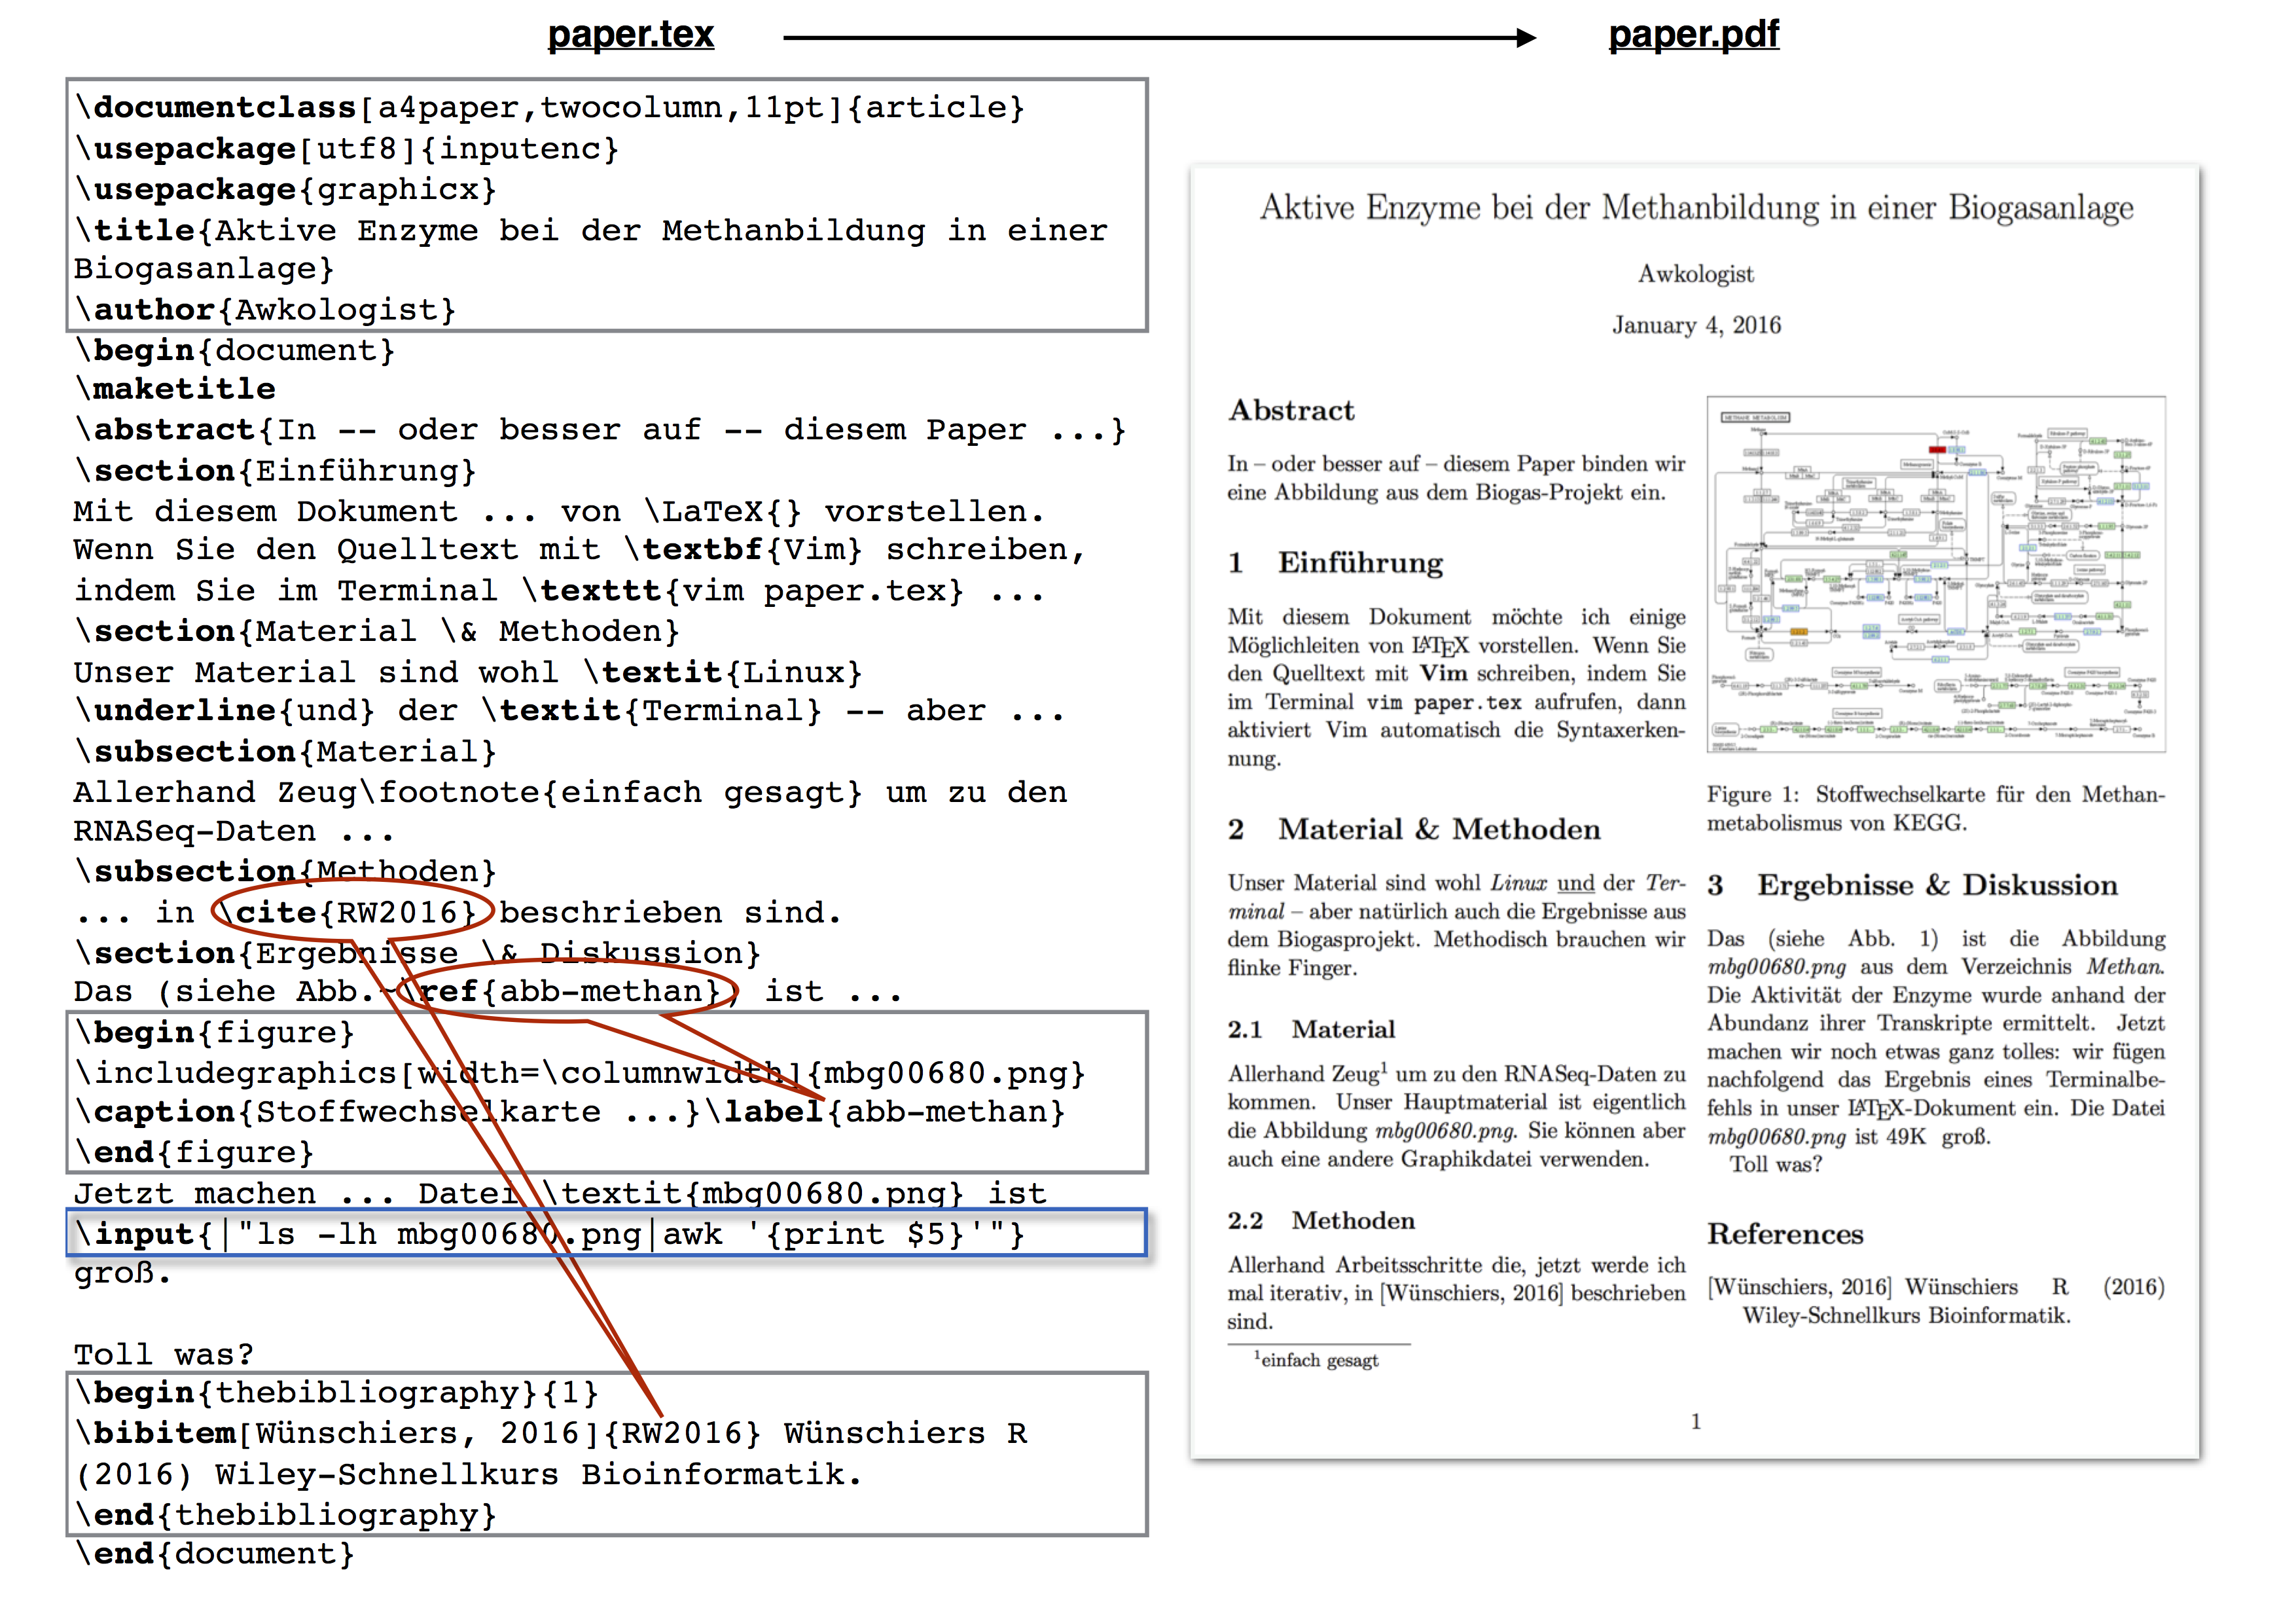
\includegraphics[width=.7\columnwidth]{fig-latex-2.png}
    \caption{Von \LaTeX{} zum PDF. Aus \citep{Wuenschiers2016}}.
    \label{fig:latex_2}
\end{figure}

Für Abbildungen verwenden Sie die Umgebung \texttt{figure}, wie im Beispiel in der Datei \textit{hsmw-vorlage-rw.tex} angewendet. 

Tabellen können beliebig komplex werden. Ein einfaches Beispiel ist in \cref{tab:mendel} zu sehen.

\begin{table}
\centering
\begin{tabular}{cccccc}
\hline
\multicolumn{3}{c}{1. Versuch} &  & \multicolumn{2}{c}{2. Versuch}\\
\multicolumn{3}{c}{Gestalt der Samen} & & \multicolumn{2}{c}{Färbung }\\
& & & & \multicolumn{2}{c}{des Albumens}\\
Pflanze & rund & kantig &   &  gelb &  grün  \\
\cline{1-3} \cline{5-6} \\
1 & 45 & 12 &   &  25 &  11  \\
2 & 27 & 8 &   &  37 &  7  \\
... & ... & ... &   &  ... &  ...  \\
10 & 25 & 7 &   &  44 &  18  \\
\hline
\end{tabular}
\caption{Eine Tabelle mit Ergebnissen aus den Versuchen von Gregor Mendel \citep{Mendel1866}.}
\label{tab:mendel}
\end{table}

TexMaker bietet unter dem Menueintrag \textit{Wizard} eine Hilfe zur Erstellung von Tabellen. 

\chapter{Referenzen im Text}
\label{cha:refs}
Wenn in Kapiteln, Abschnitten, Tabellen- oder Abbildungsumgebungen usw. mit \verb+\label{name}+ ein Label definiert wird, kann auf dieses mit \verb+\cref{XXX}+ im Text verwiesen werden. Da das Paket \textit{cleverref} verwendet wird erkennt LaTeX, wo sich das Label befindet und verwendet entsprechen 'Kapitel XXX' oder 'Abbildung XXX'. Im Englischen wird entsprechen 'chapter XXX' oder 'figure XXX' verwendet.

\alertinfo{Damit die Referenzen korrekt gesetzt werden, müssen Sie in der Regel zweimal hintereinander das PDF erzeugen (kompilieren). Ansonsten erscheinen ggf. zwei Fragezeichen.}
	
\chapter{Das Literaturverzeichnis}
\label{cha:bibliography}
In das Literaturverzeichnis gehören nur "hochwertige" Literaturstellen. Wikipedia oder Webseiten von Firmen sollten Sie mit \verb+\footnote{xxx}+ als Fußnote formatieren.

Zur Erstellung eines Literaturverzeichnisses sind in der Vorlage verschiedene Vorbereitungen getroffen. Alle Literatureinträge müssen in \textit{bibtex} formatiert und in die Datei \textit{meine-literatur.bib} eingetragen ("gepastet" werden). Dabei hilft uns das Programm \href{https://www.zotero.org}{Zotero}.

\begin{figure}[h]
\centering
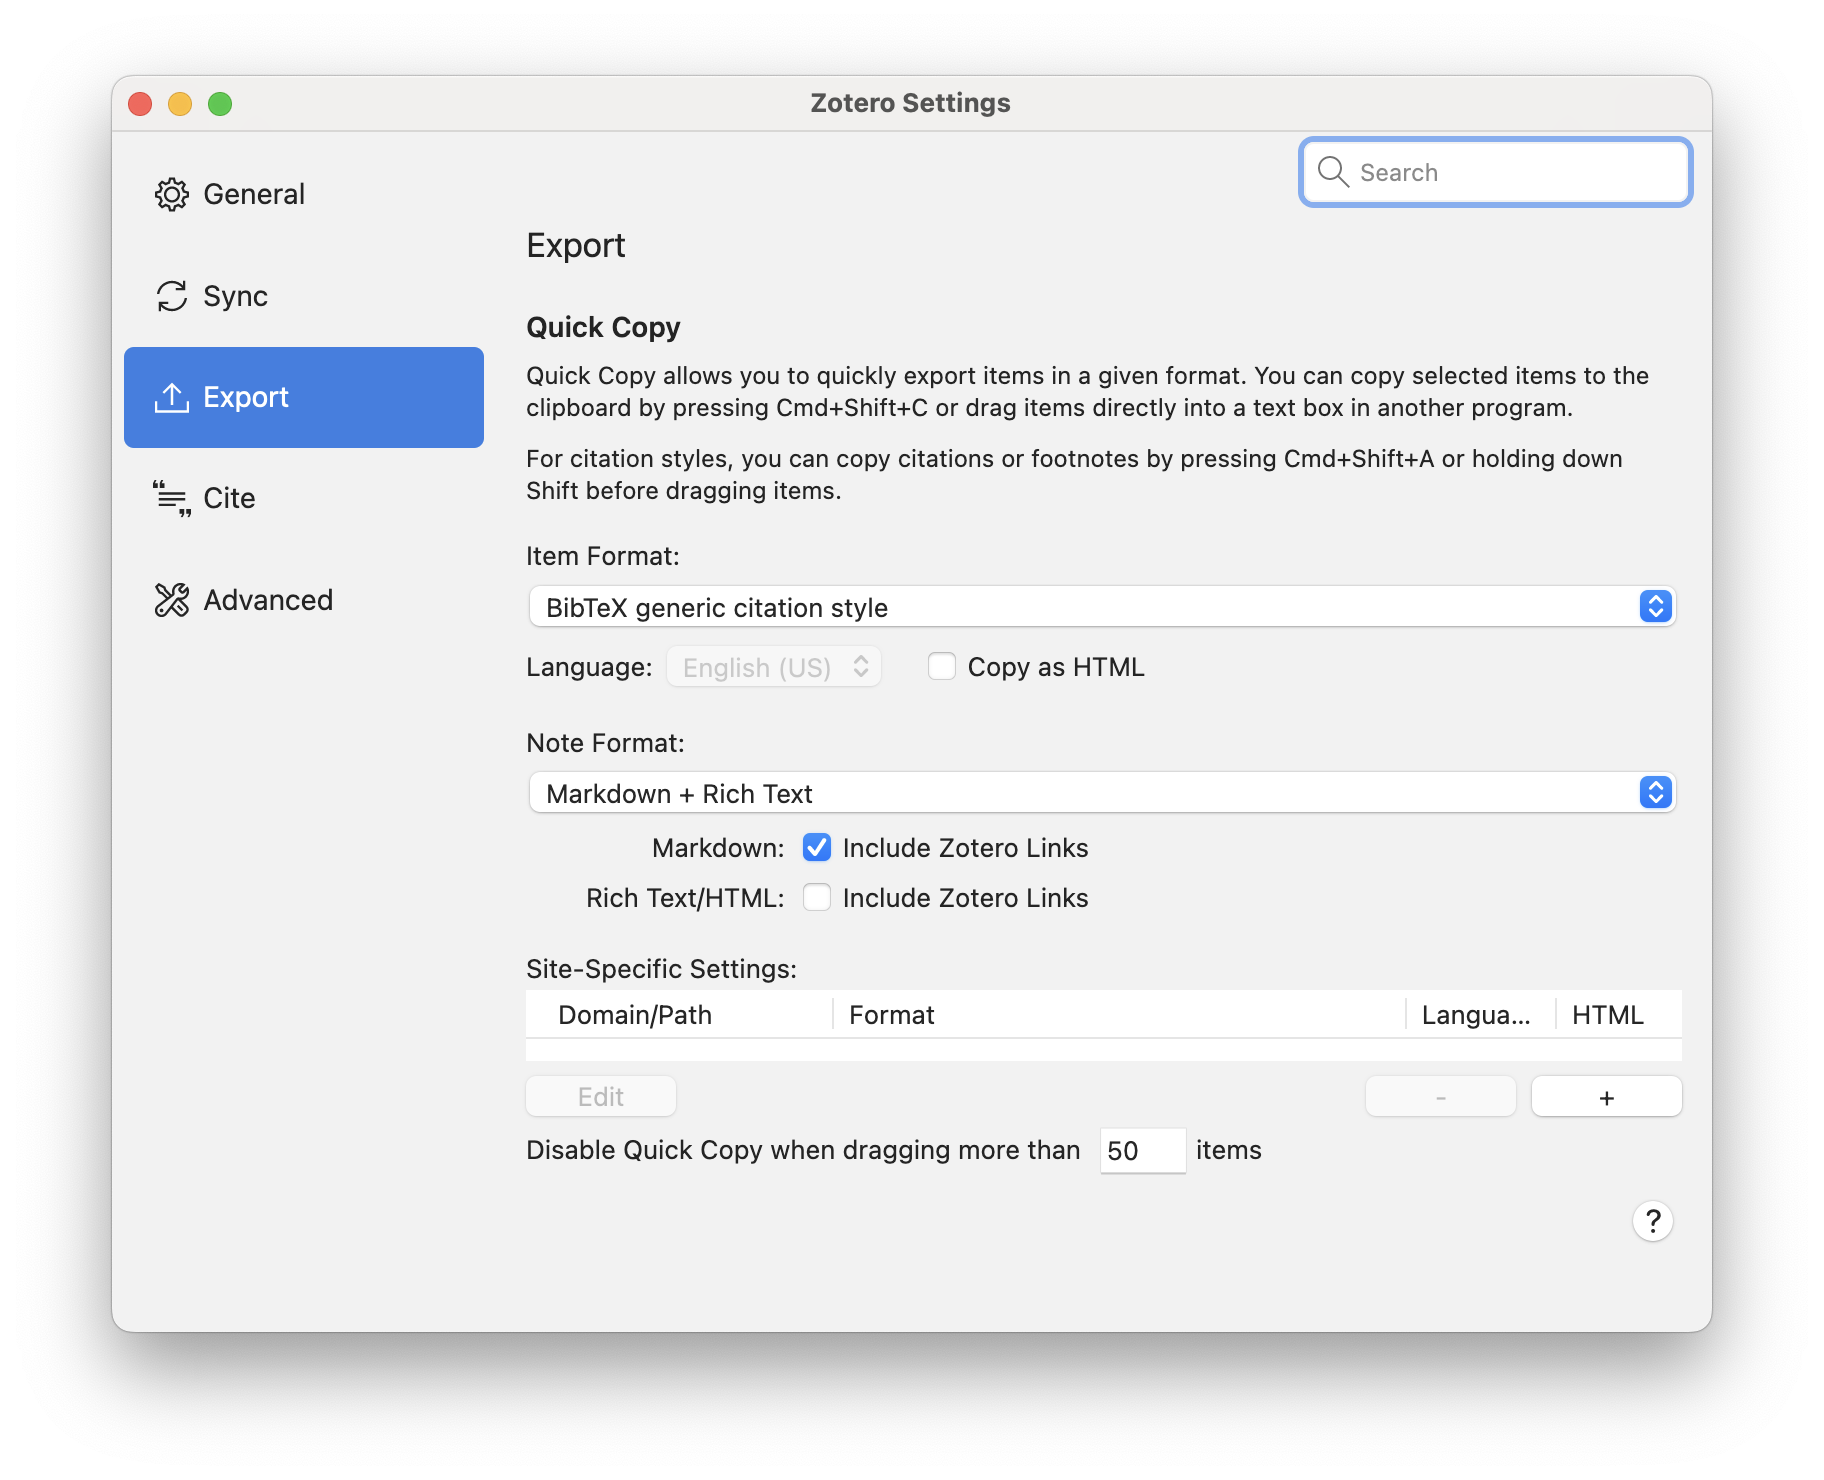
\includegraphics[width=.5\columnwidth]{zotero.png}
\caption{Wählen Sie in den Einstellungen das BibTex-Format, um Quellen korrekt formatiert in die BibTex-Datei \textit{meine-literatur.bib} einzufügen.}
\label{fig:zotero}
\end{figure}

\alertinfo{Damit die Literatur im Literaturverzeichnis erscheint, muss ggf. zweimal \texttt{pdflatex} mit \texttt{biber}ausgeführt werden.}

In \cref{tab:citing} sind ausgewählte Zitierbefehle und deren Auswirkungen in verschiedenen Zitierstilen zu sehen. Es gibt noch eine Reihe weiterer Zitierbefehle, die von \textit{biblatex} bereit gestellt werden und je nach Zielstellung sinnvoll eingesetzt werden können. Wir verwenden eigentlich ausschließlich \texttt{authoryear}.
		
\begin{table}[!htb]
\small
\centering
\caption{Beispielhafte Zitierbefehle und deren Wirkung bei ausgewählten Zitierstilen.}
\label{tab:citing}
\begin{tabular}{lll}
\toprule
\textbf{Befehl} & \textbf{\texttt{authoryear}} & \textbf{\texttt{numeric-comp}} \\
\cmidrule(r){1-1}
\cmidrule(l){2-3}
\verb|\cite{regan2008}| & Regan, 2008 & [1] \\
\verb|\cite[35]{regan2008}| & Regan, 2008, S. 35 & [1, S. 35] \\
\verb|\cite[35\psq]{regan2008}| & Regan, 2008, S. 35 f. & [1, S. 35 f.] \\
\verb|\cite[35\psqq]{regan2008}| & Regan, 2008, S. 35 ff. & [1, S. 35 ff.] \\
\verb|\cite[35-42]{regan2008}| & Regan, 2008, S. 35–42 & [1, S. 35--42] \\
\verb|\autocite{regan2008}| & (Regan, 2008) & [1] \\
\verb|\parencite{regan2008}| & (Regan, 2008) & [1] \\
\verb|\textcite{regan2008}| & Regan (2008) & Regan [1] \\
\verb|\citeauthor{regan2008}| & Regan & Regan \\
\bottomrule
\end{tabular}
\end{table}

Hier ist mal ein Paper von meiner Gruppe: \cite{Wappler_2024}. Ziemlich viele Autoren (274) hat das Paper zum humanen Genom \citep{Venter_2001}

Es ist in den meisten Befehlen auch möglich mehrere Quellen gemeinsam anzugeben, indem deren \textit{Label} entweder mit Komma (und ohne zusätzliches Leerzeichen) einfach in den bekannten Befehl eingefügt werden (z.\,B. \verb|\cite{regan2008,stamp2007}|) oder die Mehrzahl-Befehle (z.\,B. \verb|\cites{regan2008}{stamp2007}|) verwendet werden. Letzteres ist immer dann sinnvoll, wenn beispielsweise Seitenzahlen mit angegeben werden sollen.

\appendix
	
\chapter{Weitere Messwerte}
Dies ist ein Beispiel für die Einbindung zusätzlicher Daten ...
